\subsection{IndoBERT}
\label{sec:indobet}

Meskipun terdapat lebih dari 200 juta pengguna bahasa Indonesia, bahasa tersebut kurang terwakili di NLP \parencite{indolem}. Sehingga, IndoBERT muncul untuk memperbaiki situasi ini. IndoBERT adalah adaptasi dari model BERT yang khusus dilatih untuk bahasa Indonesia. Mengingat keunikan dan kompleksitas bahasa Indonesia, memiliki model yang khusus dilatih untuk bahasa ini sangat penting untuk memastikan kinerja yang optimal pada tugas-tugas NLP yang berfokus pada bahasa Indonesia \parencite{indolem}.

\begin{figure}[ht]
    \centering
    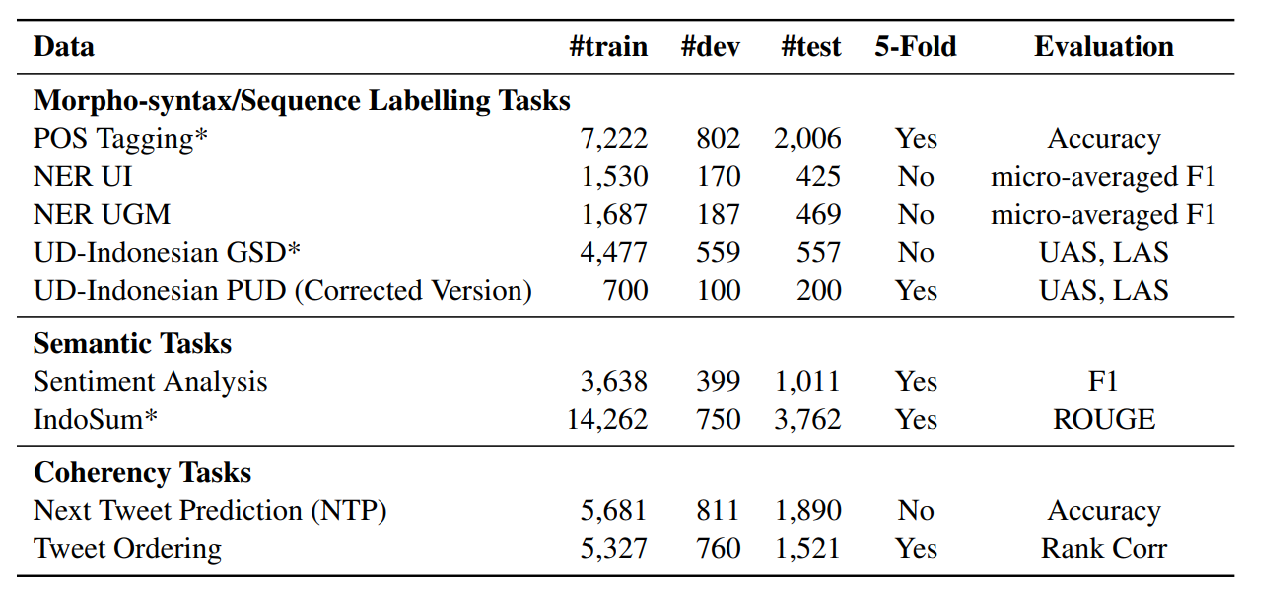
\includegraphics[width=0.8\textwidth]{chapter-2/indobert_dataset.png}
    \caption{\textit{Dataset} pada IndoBERT \parencite{indolem}}
    \label{fig:indobert_dataset}
\end{figure}

IndoBERT berbasis pada \textit{pre-trained model} BERT yang dilatih secara khusus pada \textit{dataset} berbahasa Indonesia, seperti yang bisa dilihat pada Gambar \ref{fig:indobert_dataset}. Tugas NLP yang dilatih pada IndoBERT dibagi menjadi tiga, yaitu \textit{sequence labelling}, \textit{semantic}, dan \textit{coherency}. Untuk \textit{sequence labelling} terdapat tiga tugas, yaitu \textit{part-of-speech} (POS) \textit{tagging}, \textit{named entity recognition} (NER), dan \textit{dependency parsing}. Lalu, untuk \textit{semantic} terdapat dua tugas, yaitu \textit{sentiment analysis} dan \textit{summarization}. Terakhir, untuk \textit{coherency} terdapat dua tugas, yaitu \textit{next tweet prediction} dan \textit{tweet ordering}.

\begin{figure}[ht]
    \centering
    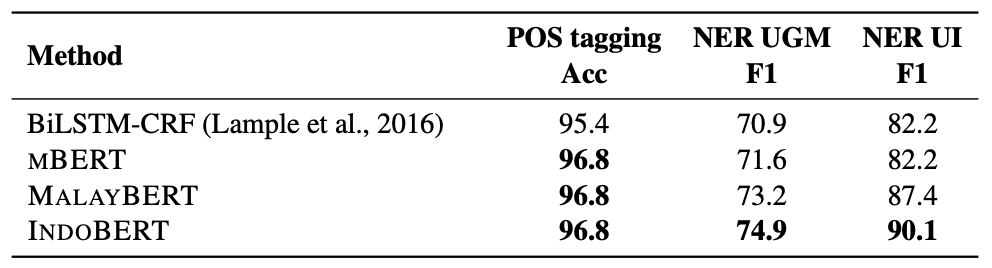
\includegraphics[width=0.8\textwidth]{chapter-2/indobert_pos.png}
    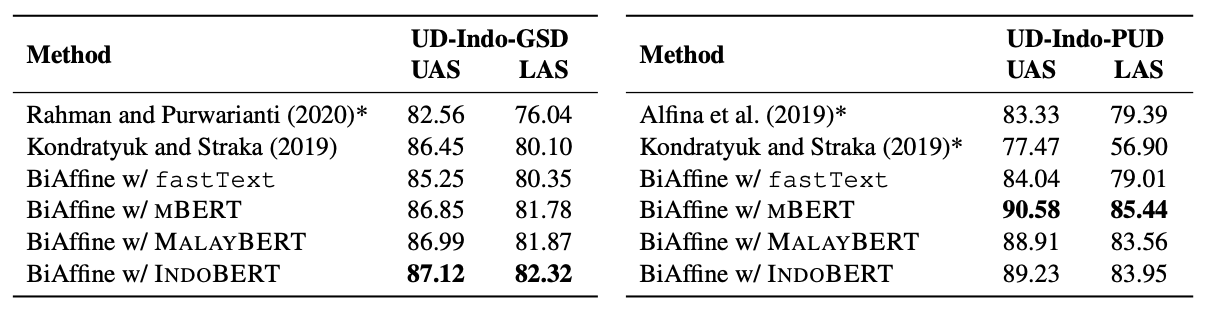
\includegraphics[width=0.8\textwidth]{chapter-2/indobert_dependency_parsing.png}
    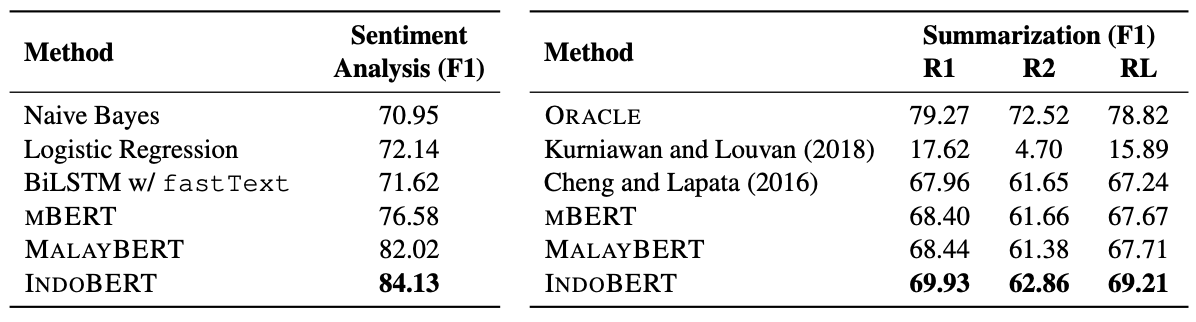
\includegraphics[width=0.8\textwidth]{chapter-2/indobert_semantic.png}
    \caption{Hasil Evaluasi IndoBERT \parencite{indolem}}
    \label{fig:indobert_evaluation}
\end{figure}

Untuk melakukan evaluasi terhadap model, dilakukan perbandingan dengan model lain. Pada penelitian ini, digunakan \textit{multilingual} BERT (mBERT) dan MalayBERT yang di-\textit{fine-tune} dengan bahasa Indonesia sebagai pembanding \parencite{indolem}. Hasilnya, IndoBERT kebanyakan unggul di setiap tugas. Selain dari tugas \textit{part-of-speech} (POS) \textit{tagging} dan \textit{next-tweet prediction} masih bisa dilakukan peningkatan \parencite{indolem}. Hasil evaluasi secara detail dapat dilihat pada Gambar \ref{fig:indobert_evaluation}.
